\section{Analisi dimensionale e stime}
Di seguito faremo delle stime di grandezze fisiche basate sull'analisi dimensionale. A tale scopo elenchiamo alcune costanti fondamentali della fisica, con le rispettive dimensioni e l'ordine di grandezza $ 10^{-34} \, \si{kg^2} $ $ \si{kg.m.s^{-1}} $
\begin{alignat*}{3}
& m_e && = [M] && \quad \sim 10^{-30} \, \si{kg} \\
& m_p && = [M] && \quad \sim 10^{-27} \, \si{kg} \\
& \hbar && = [M] [L]^2 [T]^{-1} && \quad \sim 10^{-34} \, \si{kg.m^{2}.s^{-1}} \\
& e^2 && = [M] [L]^3 [T]^{-2} && \quad \sim 10^{-28} \, \si{kg.m^3.s^{-2}} \\
& c && = [M] [T]^{-1} && \quad \sim 10^8 \, \si{m.s^{-1}} \\
& G && = [M]^{-1} [L]^3 [T]^{-2} && \quad \sim 10^{-10} \, \si{kg^{-1}.m^3.s^{-2}}
\end{alignat*}
dove $ e^2 $ è definita come $ q_e^2 / (4 \pi \epsilon_0) $. Risulterà inoltre particolarmente utile la seguente cotante adimensionale \[ \alpha = \frac{e^2}{\hbar c} \sim 10^{-2}.\]

\begin{enumerate}
	\item \emph{Stimare del raggio di Bohr $ r_B $ e dell'energia dell'elettrone}. \\
	È ragionevole pensare che il raggio di orbita dell'elettrone nell'atomo di idrogeno dipenda da $ m_e $, $ e^2 $ e $ \hbar $ ovvero che \[r_B \propto m_e^{\alpha} \, (e^2)^{\beta} \,  \hbar^{\gamma}.\] Per determinare gli esponenti dobbiamo fare in modo che la quantità di sinistra abbia le dimensioni di una lunghezza
	\[[M]^{\alpha}[M]^{\beta}[M]^{\gamma}[L]^{3\beta}[L]^{2\gamma}[T]^{-2\beta}[T]^{-\gamma} = [L]^1\]
	ovvero dobbiamo risolvere il sistema
	\[
	\begin{cases*}
	\alpha + \beta + \gamma = 0 \\
	3\beta + 2\gamma = 1 \\
	-2\beta - \gamma = 0	 
	\end{cases*}
	\qquad \Rightarrow \qquad
	\begin{cases*}
	\alpha = -1 \\
	\beta = -1 \\
	\gamma = 2 
	\end{cases*}\]
	Scriveremo quindi che 
	\begin{equation}
	r_B \sim \frac{\hbar^2}{m_e e^2} = \alpha \frac{\hbar}{m_e c} \sim 10^{-10} \, \si{m}.
	\end{equation}
	L'energia dell'elettrone èstimabile attraverso l'energia potenziale coulombiana a distanza $ r_B $ dal nucleo
	\begin{equation}
	U_e \sim \frac{e^2}{r_B} \sim \frac{e^4 m_e}{\hbar^2} = \alpha^2 m_e c^2 \sim 10^{-16} \, \si{J}.
	\end{equation}
	\item \emph{Stimare la velocità orbitale dell'elettrone} \\
	Possiamo stimare la velocità dell'elettrone passando per l'energia cinetica $ K \sim m_e v^2 $ da cui 
	\begin{equation}
	\alpha^2 m_e c^2 \sim m_e v^2 \quad \Rightarrow \quad v \sim \alpha c \sim 10^{-6} \, \si{m.s^{-1}}.
	\end{equation}
	\item \emph{Stimare la densità media della materia} \\
	\begin{equation}
	\rho = \frac{m}{V} \sim \frac{m_p}{r_B^3} \sim \frac{m_p m_e^3 c^3 \alpha^3}{\hbar^3} \sim 10^3 \, \si{kg.m^{-3}}
	\end{equation}
	\item \emph{Dare una stima del raggio massimo di un pianeta roccioso} \\
	Affinché un pianeta mantenga la propria integrità e non vada incontro a collasso gravitazionale, l'energia di legame degli atomi deve essere dello stesso ordine di grandezza dell'energia potenziale gravitazionale. L'energia di ionizzazione di un atomo è l'energia che serve per strappare un elettrone dall'atomo e sarà dunque dello stesso ordine di grandezza di $ U_e $, dunque $ E_{i} \sim \alpha^2 m_e c^2 $. Tale energia è molto più grande dell'energia che serve per rompere un legame molecolare: una stima ragionevole è che l'energia di legame sia circa un centesimo dell'energia di ionizzazione \[E_{leg} \sim \frac{1}{100} E_{i} \sim \frac{1}{100} \alpha^2 m_e c^2.\] Detto $ R $ il raggio del pianeta, il numero di atomi sarà circa $ N \sim \frac{\rho R^3}{m_p} $. L'energia potenziale gravitazionale del pianeta sarà invece \[E_G \sim \frac{G M^2}{R} \sim G \rho^2 R^5.\] Per trovare il raggio del pianeta dobbiamo quindi imporre che 
	\begin{equation}
	E_G \sim N \cdot E_{leg} \qquad \Rightarrow \qquad R \sim \frac{\hbar^3}{100 \cdot \alpha G m_p^2 m_e^2 c} \sim 10^7 \, \si{m}
	\end{equation}
	\item \emph{Stimare l'energia media per nucleone. Quanta energia è estraibile da 1 \si{kg} di Uranio?} \\
	Assumendo che il ncleo abbia densità costante $ \rho_n $, indicato con $ R_n $ il raggio del nucleo e con $ A $ il numero di massa (neutroni + protoni) si ha 
	\begin{equation}
	\frac{4}{3} \pi R_n^3 \rho_n \sim A m_p \quad \Rightarrow \quad R_n \sim R_0 A^\frac{1}{3}
	\end{equation}
	dove $ R_0 \sim 10^{-15} \, \si{m} = 1 \, \si{fermi} $ è il una stima del raggio dell'atomo di idrogeno ($ A = 1 $). \\
	L'energia dell'atomo sarà la somma di due contributi 
	\begin{itemize}
		\item \emph{energia potenziale columbiana}: poiché solo i protoni sono portatori di carica nel nucleo pari a $ q_e $, detto $ Z $ il numero atomico (numero di protoni), si ha \[U_e \sim \frac{Z^2 e^2}{R_n}.\]
		\item \emph{energia associata all'interazione forte}: poiché l'interazione forte è la stessa per neutroni e protoni essa sarà proporzionale al numero di massa $ A $ (e non solo da $ Z $); inoltre poiché sappiamo che è un'interazione a corto raggio vuol dire che in media un protone interagisce sono con i protoni con cui è a contatto dunque sarà proporzionale a $ A^1 $. In definitiva
		\[U_f \sim - E_f A\]
		dove il segno negativo sta ad indicare che è una forza attrattiva. $ E_f $ è una costante di proporzionalità che dobbiamo stimare: il numero massimo di nucleoni in un atomo stabile è circa $ Z_m \sim 10^2 $; ciò vuol dire che per $ Z \sim Z_m $ l'interazione forte (attrattiva) e l'interazione coulombiana (repulsiva) si equilibrano. Stimando $ A_m \sim 2 Z_m \sim Z_m $ e usando la stima sul raggio troviamo \[\frac{Z_m^2 e^2}{R_n} \sim E_f A_m \quad \Rightarrow \quad E_f \sim \frac{e^2 Z_m^\frac{2}{3}}{R_0} \sim \frac{\alpha \hbar c}{R_0} Z_m^\frac{2}{3} \sim 10^{-12} \, \si{J} \sim 10 \, \si{MeV}.\]
		Alla stima dell'$ U_f $ dobbiamo tuttavia aggiungere un termine correttivo: infatti non tutti i nucleoni interagiscono tra di loro ma quelli sulla superficie interagiscono in modo minore. La correzione sarà proporzionale al numero di nucleoni sulla superficie ovvero ad $ A^\frac{2}{3} $. La costante di proporzionalità sarà circa la stessa $ E_s \sim E_f $. In definitiva \[U_f \sim - E_f A + E_s A^\frac{2}{3}.\]		
	\end{itemize}
	Stimando in generale $ A \sim Z $ possiamo dare una stima dell'energia del nucleo
	\begin{equation}
	U \sim \frac{Z^2 e^2}{R_n} - E_f A + E_s A^\frac{2}{3} \sim E_c A^\frac{5}{3} - E_f A + E_s A^\frac{2}{3}
	\end{equation}
	dove $ E_c \sim \frac{e^2}{R_0} \sim \frac{\alpha \hbar c}{R_0} \sim 10^{-13} \, \si{J} $. L'energia per nucleone è quindi
	\begin{equation}
	\frac{U}{A} \sim E_c A^\frac{2}{3} + E_s \frac{1}{A^\frac{1}{3}} - E_f
	\end{equation}
	Un grafico approssimativo dell'energia per nucleone è dato nella Figura \ref{fig: SEMF per nucleon}. Notiamo incidentalmente che il grafico ha un minimo per ?Z = 26?. \\
	Nella fissione dell'$ \prescript{235}{}{U} $ l'atomo si scinde in due atomi $ U_1 $ e $ U_2 $ con $ A_U \sim 2 A_{U_1,2} $. L'energia liberata dalla fissione di un atomo di Uranio 238 è quindi \[\Delta E \sim U(235) - 2 U(118) \sim 10^{-10} \, \si{J} \sim 1 \, \si{GeV}.\] L'energia liberata dalla fissione di 1 \si{kg} di $ \prescript{235}{}{U} $ sarà quindi $ \Delta E (1 \si{kg}) \sim 4 N_A \Delta E \sim 10^14 \si{J} $.
	\begin{figure}[h]
		\centering
		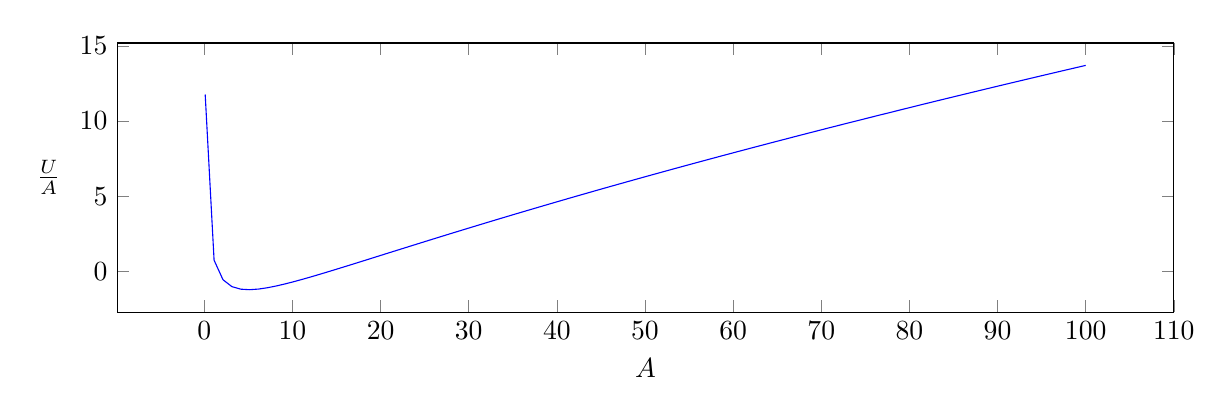
\begin{tikzpicture}% function
		\begin{axis}[xlabel = {$ A $}, ylabel = {$ \frac{U}{A} $}, ylabel style={rotate=-90}, domain = 0.1 : 100, width=15cm,
		height=5cm]
		\addplot [samples=100, blue] {x^(2/3) + 10*x^(-1/3) - 10};
		\end{axis}
		\end{tikzpicture}
		\caption{Energia del nucleo per nucleone}
		\label{fig: SEMF per nucleon}
	\end{figure}
\end{enumerate}

\section{Asta vincolata rotante}
\begin{testo}
	Un'asta vincolata in un punto si muove di sul piano con velocità angolare $ \omega $ costante.
	\begin{enumerate}
		\item Studiare il moto di un corpo di massa $ m $ vincolato a muoversi lungo l'asta.
		\item Studiare lo stesso sistema se l'asta è disposta in verticale e quindi interviene la fora di gravità
	\end{enumerate}
\end{testo}
\smallskip
\begin{sol}
	Studiamo il problema in coordinate polari. 
	\begin{enumerate}
		\item Scriviamo $ \vec F = m \vec a $ in coordinate polari. Sul corpo agisce soltanto la reazione vincolare dell'asta $ \vec R = R \vers{\theta} $ quindi
		\[ m ((\ddot r - r \dot \theta^2)\vers{r} + (r \ddot{\theta} + 2 \dot{r} \dot{\theta}) \vers{\theta}) = R \vers{\theta}
		\qquad \Rightarrow \qquad 
		\begin{cases*}
		m(\ddot r - r \dot \theta^2) = 0 \\
		m(r \ddot{\theta} + 2 \dot{r} \dot{\theta}) = R 
		\end{cases*}.\]
		In questo problema poiché l'asta si muove di velocità angolare costante lungo $ \vers{\theta} $ allora $ \dot{\theta} = \omega $ e $ \ddot{\theta} = 0 $. Le equazioni del moto diventano quindi
		\begin{align}
		\ddot{r} & = \omega^2 r \label{eqn: r}\\
		R & = 2 m \omega \dot{r} \label{eqn: theta} 
		\end{align}
		L'equazione \eqref{eqn: r} è un'equazione differenziale lineare ordinaria del secondo ordine che ha come soluzione un'esponenziale con due parametri liberi
		\begin{equation} \label{eqn: sol generale r}
			r(t) = A e^{\omega t} + B e^{- \omega t}
		\end{equation}
		Aggiungendo le condizioni iniziali $ r(0) = r_0 $ e $ \dot{r}(0) = v_0 $ possiamo determinare le costanti $ A $ e $ B $
		\[\begin{cases*}
		A + B = r_0 \\
		\omega A - \omega B = v_0
		\end{cases*}
		\qquad \Rightarrow \qquad 
		\begin{cases*}
		A = \frac{\omega r_0 + v_0}{2 \omega} \\
		B = \frac{\omega r_0 - v_0}{2 \omega}
		\end{cases*}\]
		Dunque la legge oraria del corpo lungo $ \vers{r} $ sarà 
		\begin{equation} \label{eqn: sol particolare r}
		r(t) = \frac{\omega r_0 + v_0}{2 \omega} e^{\omega t} + \frac{\omega r_0 - v_0}{2 \omega} e^{- \omega t}
		\end{equation}
		mentre lungo $ \vers{\theta} $, posto $ \theta(0) = \theta_0 $, è 
		\begin{equation} \label{eqn: sol particolare theta}
		\theta (t) = \theta_0 + \omega t
		\end{equation}
		La reazione vincolare $ \vec R $ sarà invece 
		\begin{equation} \label{eqn: reazione}
		\vec R = m [(\omega r_0 + v_0) e^{\omega t} + (\omega r_0 - v_0) e^{- \omega t}] \vers{\theta}.
		\end{equation}
		\item In presenza di un campo gravitazionale il corpo è anche soggetto alla forza peso $ \vec P = - m g \vers{y} = - m g \cos(\theta) \vers{r} - m g \sin(\theta) \vers{\theta} $. Poiché l'asta si muove sempre di moto circolare uniforme si avrà di nuovo, posto per semplicità $ \theta_0 = 0 $, $ \theta(t) = \omega t $, $ \dot{\theta} = \omega $ e $ \ddot{\theta} = 0 $. Le equazioni del moto diventano quindi
		\begin{align}
		\ddot{r} - \omega^2 r & = - g \sin (\omega t) \label{eqn: r con g} \\
		R & = 2 m \omega \dot{r} + m g \sin(\omega t) \label{eqn: theta con g} 
		\end{align}
		Questa volta l'equazione \eqref{eqn: r con g} è un'equazione differenziale non omogenea, la cui soluzione è data dalla somma dell'equazione che risolve l'omogenea associata (equazione \eqref{eqn: sol generale r}) e di una soluzione particolare della non omogenea. Provando con la soluzione particolare $ r_p(t) = K \sin(\omega t) $ troviamo che $ K = \frac{g}{2 \omega^2} $. La soluzione è quindi
		\begin{equation}
		r(t) = A e^{\omega t} + B e^{- \omega t} + \frac{g}{2 \omega^2} \sin(\omega t). 
		\end{equation}
		Poste le condizioni iniziali $ r(0) = r_0 $ e $ \dot{r}(0) = v_0 $ troviamo $ A = \frac{\omega r_0 + v_0 + \frac{g}{2\omega}}{2 \omega} $ e $ B = \frac{\omega r_0 - v_0 - \frac{g}{2\omega}}{2 \omega} $ da cui 
		\begin{equation}
		r(t) = \frac{\omega r_0 + v_0 + \frac{g}{2\omega}}{2 \omega} e^{\omega t} + \frac{\omega r_0 - v_0 - \frac{g}{2\omega}}{2 \omega} e^{- \omega t} + \frac{g}{2 \omega^2} \sin(\omega t).
		\end{equation}
	 	\end{enumerate}
\end{sol}

\section{Corpo soggetto alla forza di Lorentz}
\begin{testo}
	Un corpo di massa $ m $ è soggetto ad una forza $ \vec F = - e (\vec E + \frac{\vec v}{c} \times \vec B) $ dove $ \vec E = (E_0, 0, 0) $ e $ \vec B = (0, 0, B_0) $.
	\begin{enumerate}
		\item Quali condizioni iniziali bisogna imporre affinché il moto avvenga nel piano $ xy $?
		\item In tale caso, studiare il moto sapendo che $ \vec{r}(0) = (0, 0, 0) $ e $ \dot{\vec{r}}(0) = (0, v_y, 0) $.   
	\end{enumerate}
\end{testo}
\begin{sol}
	\begin{enumerate}
		\item Affinché il moto avvenga nel piano $ xy $ dobbiamo imporre che si abbia
		\[\begin{cases}
			z(0) = 0 \\
			\dot{z}(0) = 0 \\
			\ddot{z}(0) = 0
		\end{cases}\]
		Infatti in tal modo il corpo non è soggetto a forze e accelerazioni lungo $ z $.
		\item Studiamo il moto del corpo nel piano cartesiano $ xy $. $ \vec F = m \vec a $ proiettata lungo la direzione $ \vers{x} $ e la direzione $ \vers{y} $ diventa
		\begin{align}
		m \ddot{x} & = - e (E_0 + \frac{\dot{y}}{c} B_0) \label{eqn: x} \\
		m \ddot{y} & = e \frac{\dot{x}}{c} B_0 \label{eqn: y}
		\end{align}
		Tali espressioni sono \emph{accoppiate} e per separare le variabili $ x $ e $ y $ integriamo una volta l'equazione \eqref{eqn: y} ottenendo
		\begin{equation} \label{eqn: integrazione di y''}
		\dot{y} = v_y + \frac{e B_0}{mc} x
		\end{equation}
		e sostituendo nell'equazioen \eqref{eqn: x}, posto $ \omega = \frac{e B_0}{mc} $ , otteniamo l'equazione del moto armonico
		\begin{equation}
		\ddot{x} = - \frac{e}{m} \Bigl (E_0 + \frac{v_y B_0}{c} + \frac{e B_0^2}{mc^2} x \Bigr) = - \omega^2 x - \omega v_y - \omega c \frac{E_0}{B_0} = -\omega^2 \Bigl ( x + \frac{v_y}{\omega} + \frac{c E_0}{\omega B_0} \Bigr ).
		\end{equation}
		La soluzione generale dell'equazione differenziale è dunque
		\begin{equation} \label{eqn: sol generale x}
			x(t) = A_1 \sin(\omega t) + A_2 \cos(\omega t) - \frac{v_y}{\omega} - \frac{c E_0}{\omega B_0}.
		\end{equation}
		Imponendo le condizioni iniziali troviamo che $ A_1 = 0 $ e $ A_2 = \frac{v_y}{\omega} + \frac{c E_0}{\omega B_0} $ da cui la soluzione particolare è 
		\begin{equation} \label{eqn: sol particolare x}
		x(t) = \frac{v_y B_0 + c E_0}{\omega B_0}(\cos(\omega t) - 1).
		\end{equation}
		Sostituendo $ x(t) $ nella \eqref{eqn: integrazione di y''} e integrando nuovamente, posto $ \alpha = \frac{v_y B_0 + c E_0}{\omega B_0} $ otteniamo
		\begin{equation}
			\dot{y} = v_y + \omega \alpha (cos(\omega t) - 1) \quad \Rightarrow \quad y(t) = (v_y - \alpha \omega) t + \alpha \sin(\omega t)
		\end{equation}
		Il moto è quindi descritto dall'equazione parametrica
		\begin{equation}
		\begin{cases}
			x(t) = \alpha (cos(\omega t) - 1) \\
			y(t) = (v_y - \alpha \omega) t + \alpha \sin(\omega t)
		\end{cases}
		\end{equation}
	\end{enumerate}
\end{sol}

\section{Fune massiva appesa verticalmente}
\begin{testo}
	Una fune di lunghezza $ L $ e massa per unità di lunghezza $ \rho $ viene appesa verticalmente ad un'estremità. Trovare la tensione nella fune al variare della distanza dall'estremo libero. 
\end{testo}
\begin{sol}
	Imponiamo la condizione di equilibrio elemento $ \dif{m} $ tra $ y $ e $ y + \dif{y} $ 
	\begin{gather*}
	T(y + \dif{y}) - T(y) - \dif{m} g = 0 \\
	\d T(y) = \rho g \dif{y}
	\end{gather*}
	 che è un'equazione differenziale a variabili separabili. Integrando troviamo
	\begin{equation}
	\int_{0}^{T(y)} \d T' = \rho g \int_{0}^{y} \d y' \qquad \Rightarrow \qquad	T(y) = \rho g y
	\end{equation}
	Dove nell'integrazione abbiamo sfruttato il fatto che $ T(0) = 0 $. 
\end{sol}

\section{Fune massiva in equilibrio}
\begin{testo}
	Quale deve essere la lunghezza di una fune di massa per unità di lunghezza $ \rho $ affinché essa possa restare in equilibrio verticale "sulla Terra"?
\end{testo}
\begin{sol}
	Indichiamo con $ a = \frac{r}{R_T} $ il rapporto tra la distanza di un punto dal centro della Terra e il raggio terrestre. Considerando un elemento infinitesimo della fune di lunghezza $ \dif{r} = R_T \dif{a} $ a distanza $ r = R_T a $ dal centro della Terra, dobbiamo imporre l'equilibrio tra la forza gravitazionale $ F_G = - G \frac{M_T \dif{m} }{r^2} $, la forza centrifuga $ F_c = \omega^2 r \dif{m} $, dove $ \omega $ è la velocità rotazionale terrestre, e la tensione in $ r $ e in $ r + \dif{r} $
	\begin{gather*}
	T(r + \dif{r}) - T(r) = G \frac{\frac{4}{3} \pi R_T^3 \rho_T \,  \rho R_T \dif{a} }{R_T^2 a^2} - \omega^2 R_T a \rho R_T \dif{a} \\
	\d T = \rho R_T^2 \Bigl( \frac{4 \pi G \rho_T}{3 a^2} - \omega^2 a \Bigr) \dif{a}
	\end{gather*}
	Ricordando ora che dalla condizione di orbita geostazionaria $ m \omega r = G \frac{m M_T}{r^2} $ ricaviamo che $ a_g^3 = \frac{r_g}{R_T} = \frac{4 \pi G \rho_T}{3\omega^2} (\frac{R_T}{r})^3 $ possiamo riformulare l'ultima equazione come 
	\[\d T = \rho R_T^2 \omega^2 \Bigl( \frac{a_g^3}{a^2} - a \Bigr) \dif{a}\]
	che integrata fornisce 
	\begin{align*}
	T(a) & = \rho R_T^2 \omega^2  \int \Bigl( \frac{a_g^3}{a^2} - a \Bigr) \dif{a} = \\
	& = \rho R_T^2 \omega^2 \Bigl( - \frac{a_g^3}{a} - \frac{a^2}{2} \Bigr) + c
	\end{align*}
	Per determinare la costante $ c $ imponiamo la condizione $ T(1) = 0 $ ovvero che la tensione a contatto con il suolo sia nulla. In tale modo otteniamo $ c = a_g^3 + \frac{1}{2} $ da cui infine
	\begin{equation}
	T(a) = \rho R_T^2 \omega^2 \Bigl( a_g^3 \Bigl(1 - \frac{1}{a} \Bigr) - \frac{1 - a^2}{2} \Bigr).
	\end{equation}
	La condizione $ T(a) = 0 $ ci darà l'altro punto dove la tensione è nulla, ovvero dove termina la fune
	\begin{gather*}
	T(a) = \rho R_T^2 \omega^2 (a - 1) \Bigl( - \frac{a_g^3}{a} + \frac{1 + a}{2} \Bigr) \\
	a = 1 \vee a^2 + a - 2 a_g^3 = 0
	\end{gather*}
	da cui ricaviamo infine la lunghezza della fune
	\begin{equation}
	a = \frac{\sqrt{8 a_g^3 + 1} - 1}{2} \qquad \Rightarrow \qquad L = \frac{\sqrt{8 a_g^3 + 1} - 1}{2} R_T - R_T \approx 22 \cdot R_T
	\end{equation}
\end{sol}
